% Write the report here. You can use the nested imports via 'subimport', see the following link:
% https://www.overleaf.com/learn/latex/Management_in_a_large_project#Using_the_import_package
% You also can see an example at line n.16.

\section{Basic concepts}
We start with considering the Limit Order Book (LOB) structure. Within this paradigm of organizing an exchange, 
each person with access to trading has two opportunities: 
\begin{itemize}
    \item to express a desire to buy or sell a certain number of units of an asset at a price. In this case, the 
    exchange will "remember" his desire. The set of price-quantity pairs of assets can be aggregated by price levels and 
    depicted as at \ref{LOBpic}.
    \item to express a desire to buy or sell a certain number of units of an asset immediately. In this case, he will 
    be offered the required number of shares at the best possible price. For example, in the case of a purchase, 
    orders from the price level corresponding to the best price are first matched. If there are not enough shares 
    at that level to fill the order, the next shares are taken from the next price level and so on.
    
\end{itemize}

\begin{figure}
    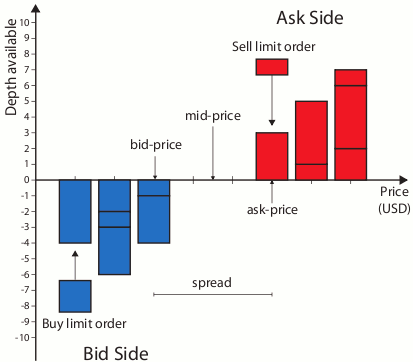
\includegraphics[scale=0.8]{fig/Graphical-representation-of-the-Limit-Order-Book.png}
    \caption{Graphical representation of the Limit Order Book}
    \label{LOBpic}
\end{figure}



So, in general, there exist 
two types of interaction with the exchange:
\begin{definition}
    A \textbf{limit order} is an order to buy or sell a security at a specific price or better. This type of order guarantees the execution price, but does not guarantee the execution itself.
\end{definition}
\begin{definition}
    A \textbf{market order} is an order to buy or sell a security immediately. This type of order guarantees that the order will be executed, but does not guarantee the execution price.
\end{definition}

Let us introduce several definitions that we will need later.
\begin{definition}
    A \textbf{bid} (price) is the highest price that a buyer (i.e., bidder) is willing to pay for the asset. We will denote bid at time $t$ as $B_t$.
    An \textbf{ask} (price) is the price a seller states they will accept. We will denote ask at time $t$ as $A_t$.
    The \textbf{bid–ask spread} $s$ is the difference between the prices quoted for an immediate sale (ask) and an immediate purchase (bid): $s = A_t - B_t$.
    The \textbf{mid-quote price}: $V_{t} = \frac{A_{t} + B_{t}}{2}$.
\end{definition}

% \begin{figure}
%     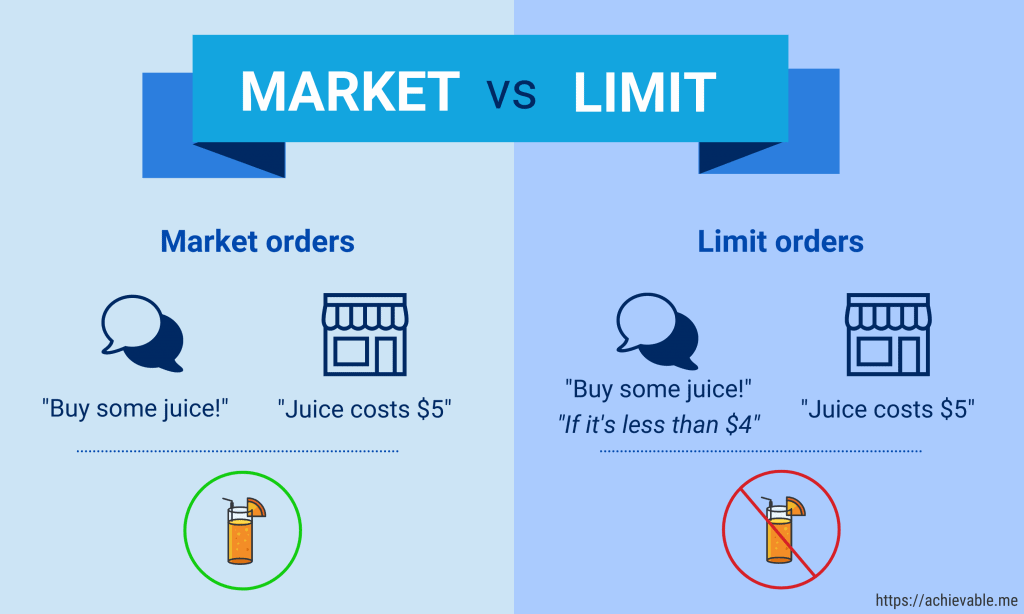
\includegraphics[scale=0.4]{fig/market-vs-limit-1024x614.png}
%     \caption{The difference between market order and limit order}
%     \label{fig:mvslim}
% \end{figure}

Now, it is clear that if one wants to sell or buy an amount of an asset large enough to have a significant 
impact on the market, he should not do it by one order: it would be very expensive, since a large order 
would remove all the upper levels in the limit order book. Therefore, in practice, all large orders are split into a large number of small ones. 
For example, one can simply divide an order into N equal parts and sell them at regular intervals (this is called TWAP).
But is there a better solution?


\section{Obizhaeva--Wang Framework}
Trying to find better solution, we consider an Obizhaeva--Wang Model model, in which terms the problem has the following form: \par
\begin{align*} \label{oEproblem}
    J_0 &= \min _{\{x_0 \cdots x_N \}} E_0 \left[ \sum _{n=0}^N [A_{t_n} + x_n /(2q)] x_n\right],  \\
    A_{t_n} &= F_{t_n} + \lambda (X_0 - X_{t_n}) + s/2 + \sum _{i=0}^{n-1} x_i \kappa e^{- \rho \tau (n - i)}.
 \end{align*}
 
Here:
\begin{itemize}
 \item The trader has to buy $\mathbf{X_0}$ units of a security over a fixed time period $[0,T]$. 
 \item $x_{t_n}$ 
 --- the trade size at $t_n = \tau n$, where $\tau = T / N$. 
 \item $X_{t_n} := X_0 - \sum _{t_k < t_n} x_{t_k}$. 
 \item $B_{t_n}$ and $A_{t_n}$ --- bid and ask prices at $t_n$. 
 \item $V_{t_n} = \frac{A_{t_n} + B_{t_n}}{2}$ 
 --- the mid-quote price; 
 \item $s$ --- the bid–ask spread.
 \item $F_t$ --- the fundamental price of the security.
 \item $q(P)$ --- the density of limit orders to sell at price $P$.
 % \item $q$, $\lambda$ and $\rho$ is a LOB density, the permanent price impact and the resiliency.
 \item Parameter $\lambda$ captures the permanent price impact.
 \item Parameter $q$ is a LOB density. 
  \item $\kappa = \frac{1}{q} - \lambda $
 \item Parameter $\rho$ captures the resiliency.
\end{itemize}

The solution to this stochastic optimal control problem was found in the article \cite{obizhaeva2013optimal}:
\begin{theorem}
    The solution to the optimal execution problem is
    \begin{multline*}
        x_n = - \frac{1}{2} \delta_{n + 1} [D_{t_n} (1 - \beta_{n + 1} e^{ - \rho \tau} + 2 \kappa \gamma_{n+1} e^{ - 2 \rho \tau}) 
         - X_{t_n} (\lambda + 2 \alpha_{n+1} - \beta_{n+1}\kappa e^{ - \rho \tau}) ], 
    \end{multline*}
    with $x_N = X_N$ and $D_t = A_t - V_t - s/2$. The expected cost for future trades under the optimal
    strategy is determined according to
    \begin{equation*}
        J_{t_n} = (F_{t_n} + s/2) X_{t_n} + \lambda X_0 X_{t_n} + \alpha_n X_{t_n} ^2 + \beta_{n} D_{t_n} X_{t_n} + \gamma_n D_{t_n}^2, 
    \end{equation*}
    where the coefficients $\alpha_{n+1}$, $\beta_{n+1}$, $\gamma_{n+1}$, and $\delta_{n+1}$ are determined recursively as follows:
    \begin{equation*}
        \alpha_{n} = \alpha_{n+1} - \frac{1}{4} \delta _{n+1} (\lambda + 2 \alpha_{n+1} - \beta_{n+1} \kappa e^{- \rho \tau})^2, 
    \end{equation*}
    \begin{multline*}
        \beta_{n} =  \beta_{n+1} e^{- \rho \tau} + \frac{1}{2} \delta _{n+1} (1 - \beta_{n+1} e^{- \rho \tau} 
         + 2 \kappa \gamma_{n+1} e^{- 2 \rho \tau}) (\lambda + 2 \alpha_{n+1} - \beta_{n+1} \kappa e^{-\rho \tau}), 
    \end{multline*}
    \begin{equation*}
         \gamma_n =   \gamma_{n+1} e^{- 2 \rho \tau} - \frac{1}{4} \delta _{n+1} (1 - \beta _{n+1} e^{- \rho \tau} 
    + 2 \gamma _{n+1} \kappa e^{- 2 \rho \tau})^2, 
    \end{equation*}
    with $\delta_{n+1} = [1/(2q) + \alpha_{n+1} - \beta_{n+1} \kappa e^{-\rho \tau} + \gamma _{n+1} \kappa ^2 e^{- 2 \rho \tau}]^{-1}$ and terminal conditions
    \begin{equation*}
        \alpha_{N} = 1/(2q) - \lambda, \;\;\;\;\;\;\; \beta_N = 1, \;\;\;\;\;\;\; \gamma_N = 0.
    \end{equation*}
\end{theorem}

In our research we will consider the limit of this problem, because it requires less amount of factors:

\begin{theorem}
    As $N \rightarrow \infty$, the optimal execution strategy becomes:
    \begin{align*}
        & \lim _{N \rightarrow \infty} x_0 = x_{t = 0} = \frac{X_0}{\rho T + 2}, \\
        & \lim _{N \rightarrow \infty} x_n / (T/N) = \dot X _t = \frac{\rho X_0}{\rho T + 2}, \;\;\;\;\;\; t \in (0, T), \\
        & \lim _{N \rightarrow \infty} x_0 = x_{t = 0} = \lim _{N \rightarrow \infty} x_n / (T/N) = x_{t=T}=  \frac{X_0}{\rho T + 2}.  %\\
    \end{align*}
    where $x_0$ is the trade at the beginning of trading period, $x_N$ is the trade at the end of trading
    period, and $\dot X _t$ is the speed of trading in between these trades.
\end{theorem}

Thus, we have an explicit form of optimal execution strategy, but to use and implement it we need to find the factors 
$\rho, \kappa$ and $\lambda$. And it is not obvious how to do that.


\section{Our methodology to find the factors}

We provide our methodology to find $\rho$. We find it, considering the time series of elements of the model 
that can be calculated from market data. As an example, we are going to consider the regression:
\begin{theorem}
        In the regression:                                                                                                                                                                                                                                                                                                                                                                                        
        \begin{equation*}
            \frac{\Delta A_{k+2}}{\Delta t_{k+2}} - \frac{\Delta A_{k+1}}{\Delta t_{k+1}} 
        = - \rho \Delta A_{k+1} + \rho \lambda x_{k+1} + (\kappa + \lambda) (\frac{x_{k+2}}{\Delta t_{k+2}} - \frac{x_{k+1}}{\Delta t_{k+1}}).
        \end{equation*}
        the coefficients $\rho, \kappa$ and $\lambda$ the same as in OW model describes the market with dynamics
        describing by series $A_k, \Delta t _k, x_k$.
\end{theorem}

        Here all the information needed can be extracted from the l3 data: 
        \begin{itemize}
            \item $\Delta A_{k}$ is an ask change after execution of the limit order with the depth $x_k$.
            \item $\Delta t_{k}$ is a time between $k$ and $k + 1$ orders of dataset.
        \end{itemize}